\section{Example: Chain Replication}

\begin{figure}[ht!]
    \centering
    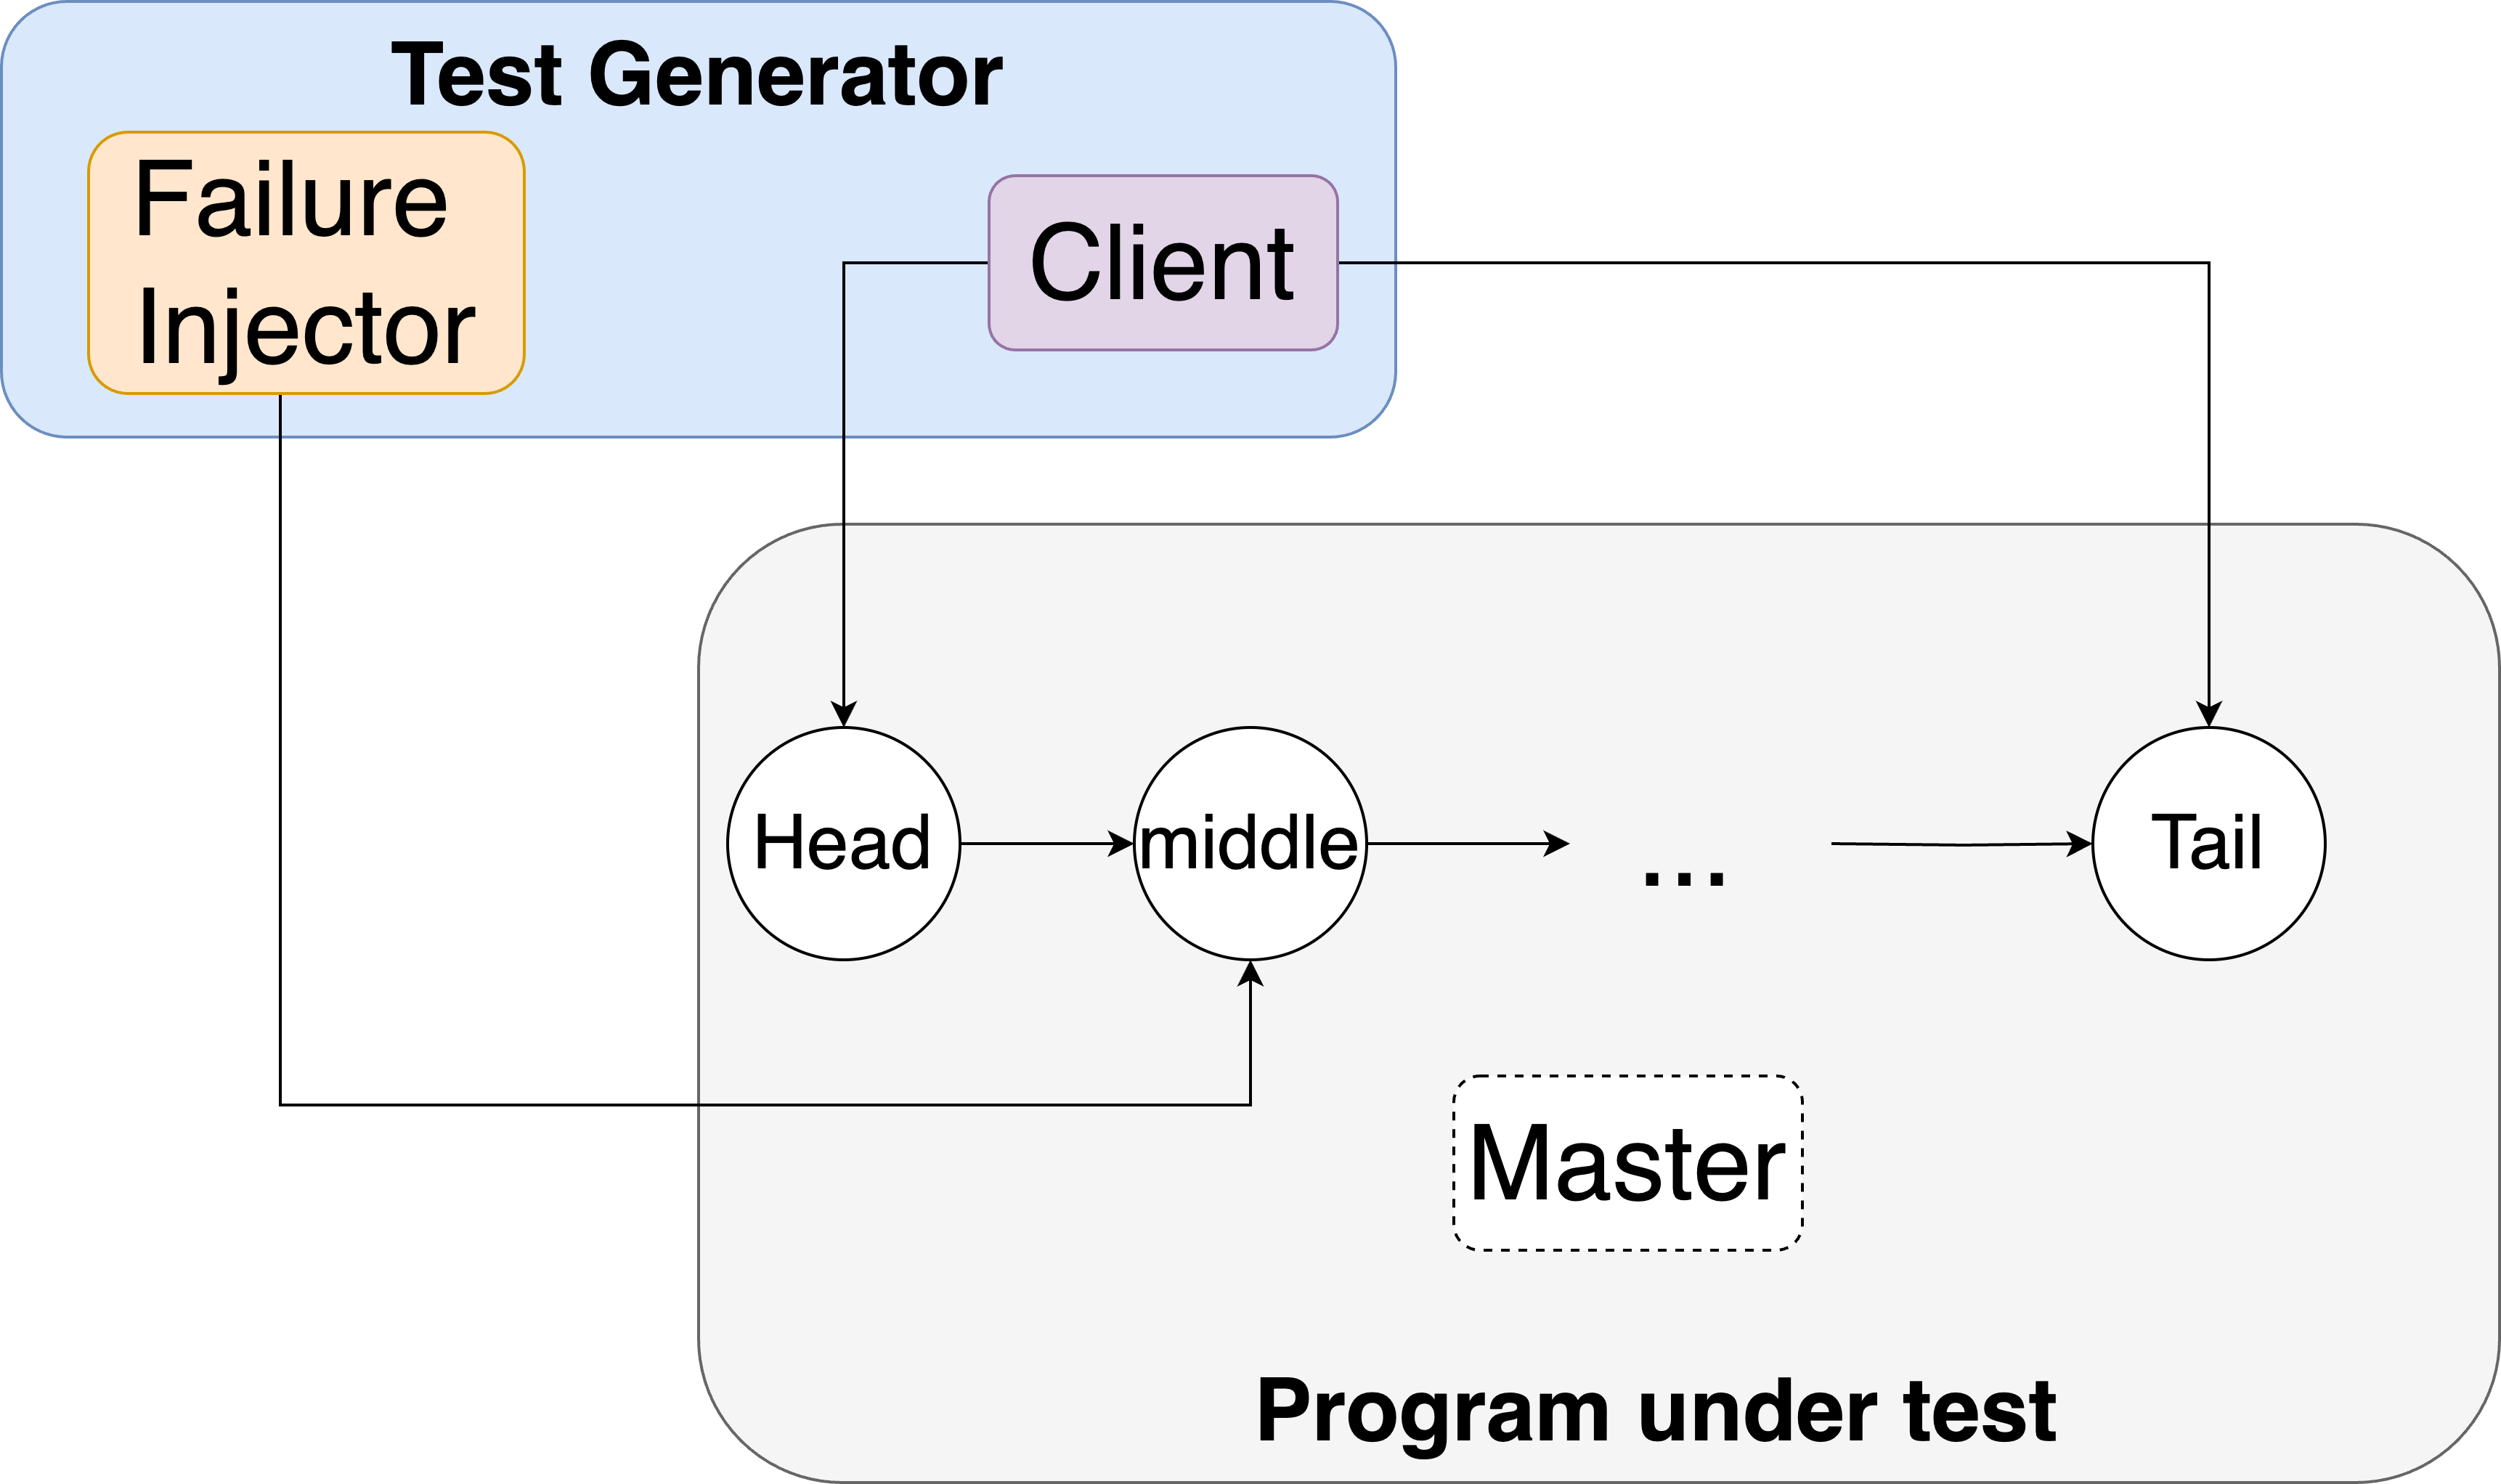
\includegraphics[width = 200pt]{figures/Chain-Replication.drawio.png}
    \caption{Chain Replication}
    \label{fig:chain-replication}
\end{figure}

Consider the Chain Replication as shown in \autoref{fig:chain-replication}, where the ``server'' program under test consists of a chain of nodes and a master node (a hidden node for environment). As it is a open system, we need to supply clients that send \Code{read} and \Code{write} requests to the server. Moreover, we also expect there is a ``failure injector'' can randomly terminate several nodes in chain to simulate the ``fail-stop'' in storage system. Note that both clients and failure injector are ``test generator'' in our open system setting, which simulate the \emph{environment} of a running server may interact with in reality.

Our automated testing framework would like to test the server against the ``strong consistency'' property, which is a safety property needed to guarantee by both test generators and servers, called \emph{global property}. Especially, for the client side, the client should send a \Code{read} request on a key has not written successfully (return with success status from server) yet. On the other hand, we also expect the client should really efficiently targeting testing the strong consistency to find bug easier, since it should: 1. write a key for at most two times 2. has a least a read request after a serials of write requests. These properties, called \emph{local properties}, is different from the global safety property (e.g., strong consistency) don't talk about the behaviors of servers, but just guide the client to explore a subset of executions the users believe are interesting. Although a client only sends no \Code{read} request is valid and may happens in reality; however, it cannot help us detect the strong consistency bug. For a desirable client, it should always make sure the message sent by itself doesn't violate the global property (then if server violates the global property means finding a bug), and also do the thing required by local property to explore subset executions which enables the users to encode domain knowledge to find bug more efficiently.

\subsection{Events in Chain Replication}

Now we introduces the observable events in chain replication example, where we unify the terminology of events and messages are events (with source and destination machine as parameters). Formally, we define events as
\begin{align*}
    ev \doteq \evp{\effop}{}{\I{source}\;\I{destination}\;\overline{x}}{\phi} 
\end{align*}\noindent
Then there are two sets of events, they are events between clients and servers, as well as events between failure injectors and servers.

\paragraph{Events between clients and servers} There are $4$ events, as shown below (the source and destination are omitted):
\begin{minted}[fontsize = \footnotesize, escapeinside=!!]{ocaml}
val writeReq: id:int -> k:Key.t -> v: Value.t -> unit
val readReq: id:int -> k:Key.t -> unit
val writeResp: id:int -> k:Key.t -> v: Value.t -> unit
val readResp: id:int -> k:Key.t -> v: Value.t -> unit
\end{minted}

where $\Code{id}$ indicates the $\Code{id}^{th}$ request send by client; the first two are request events (from clients to servers), and the last two are response events (from servers to clients).

\paragraph{Events between failure injector and servers} There are only $1$ event that is from failure injector to servers.
\begin{minted}[fontsize = \footnotesize, escapeinside=!!]{ocaml}
val shutdown: source -> destination -> unit
\end{minted}

which terminates the server node $\Code{destination}$.

\subsection{Global property}

We always use $P^{G}$ to indicate global properties. In this setting, we have two global properties, the first one is read-write safety:
\begin{align*}
    P^{G}_\text{read-write-safe} \doteq \forall \Code{key}. \evp{writeResp}{}{s\;d\;i\;k\;v}{k = \Code{key}} \weakUntilA \evp{readReq}{}{s\;d\;i\;k}{k = \Code{key}}
\end{align*}\noindent
where $\weakUntilA$ is weak until modality, and this specification involves both requests and responses. The second one is strong consistency:
{\small
\begin{align*}
    &P^{G}_\text{strong-consistency} \doteq 
    \\&\forall \Code{key}\;\Code{va}. \globalA (\neg \nextA \finalA  
    \evp{writeResp}{}{s\;d\;i\;k\;v}{k = \Code{key}} \impl  
    \\&\evp{writeResp}{}{s\;d\;i\;k\;v}{k = \Code{key} \land v = \Code{va}} \weakUntilA \evp{readResp}{}{s\;d\;i\;k\;v}{k = \Code{key} \impl v = \Code{va}})
\end{align*}}\noindent

\subsection{Local property}

{\small\begin{align*}
    &P^{L}_\text{finally-read} \doteq \evp{writeReq}{}{s\;d\;i\;k\;v}{\top}^*; \evp{readReq}{}{s\;d\;i\;k\;v}{\top}
    \\&P^{L}_\text{write-twice} \doteq \exists \Code{key}.\forall \Code{va}.\finalA (\evp{writeReq}{}{s\;d\;i\;k\;v}{k = \Code{key} \land v = \Code{va}}; \finalA \evp{writeReq}{}{s\;d\;i\;k\;v}{k = \Code{key} \land v \not= \Code{va}})
\end{align*}}\noindent
The first property indicates we should send several write request and then finally read, the second property indicates that there should be at least a key be written for at least twice.

\subsection{Translation}

Now we talk about how to translate our specification into a \Code{P} program, notice that the $P^{G}_\text{strong-consistency}$ doesn't talk about events send by the clients, thus I discuss it later.

\paragraph{Desugar specifications into Symbolic Regular Language (SRL)} We desugar the specification $P^{G}_\text{read-write-safe}$, $P^{L}_\text{finally-read}$, and $P^{L}_\text{write-twice}$ into SRL.
{\small\begin{align*}
    &P^{G}_\text{read-write-safe} \doteq \forall \Code{key}. 
    (\anyA \setminus \evp{readReq}{}{s\;d\;i\;k}{k = \Code{key}})^* \lor 
    \\&(\anyA \setminus \evp{readReq}{}{s\;d\;i\;k}{k = \Code{key}})^*; \evp{writeResp}{}{s\;d\;i\;k\;v}{k = \Code{key}};\anyA^*
    \\&P^{L}_\text{finally-read} \doteq \evp{writeReq}{}{s\;d\;i\;k\;v}{\top}^*; \evp{readReq}{}{s\;d\;i\;k\;v}{\top}
    \\&P^{L}_\text{write-twice} \doteq \exists \Code{key}.\forall \Code{va}.
    \\&\anyA^*;\evp{writeReq}{}{s\;d\;i\;k\;v}{k = \Code{key} \land v = \Code{va}};\anyA^*;\evp{writeReq}{}{s\;d\;i\;k\;v}{k = \Code{key} \land v \not= \Code{va}};\anyA^*
\end{align*}}\noindent
We also simplify the specifications into one global and one local specification:
{\small\begin{align*}
    &P^{G} \doteq \forall \Code{key}. 
    (\anyA \setminus \evp{readReq}{}{s\;d\;i\;k}{k = \Code{key}})^* \lor 
    \\&(\anyA \setminus \evp{readReq}{}{s\;d\;i\;k}{k = \Code{key}})^*; \evp{writeResp}{}{s\;d\;i\;k\;v}{k = \Code{key}};\anyA^*
    \\&P^{L} \doteq \exists \Code{key}.\forall \Code{va}. 
    \\&\evp{writeReq}{}{s\;d\;i\;k\;v}{\top}^*;\evp{writeReq}{}{s\;d\;i\;k\;v}{k = \Code{key} \land v = \Code{va}};
    \\&\evp{writeReq}{}{s\;d\;i\;k\;v}{\top}^*;\evp{writeReq}{}{s\;d\;i\;k\;v}{k = \Code{key} \land v \not= \Code{va}};\evp{writeReq}{}{s\;d\;i\;k\;v}{\top}^*;\evp{readReq}{}{s\;d\;i\;k\;v}{\top}
\end{align*}}\noindent

\paragraph{Extend the local specification with response events} We should unify the safety (overapproximate) specification as one, which needs to conjunct global and local specifications. Thus, we should first extend the local specification:
{\small\begin{align*}
    &A \doteq (\evp{writeResp}{}{...}{\top} \lor \evp{readResp}{}{...}{\top})^*
    \\&P^{L}_{extended} \doteq \exists \Code{key}.\forall \Code{va}. 
    \\&(A;\evp{writeReq}{}{s\;d\;i\;k\;v}{\top})^*;A;\evp{writeReq}{}{s\;d\;i\;k\;v}{k = \Code{key} \land v = \Code{va}};
    \\&(A;\evp{writeReq}{}{s\;d\;i\;k\;v}{\top})^*;A;\evp{writeReq}{}{s\;d\;i\;k\;v}{k = \Code{key} \land v \not= \Code{va}};
    \\&(A;\evp{writeReq}{}{s\;d\;i\;k\;v}{\top})^*;A;\evp{readReq}{}{s\;d\;i\;k\;v}{\top};A
\end{align*}}\noindent

\paragraph{Construct the global safety and local completeness specification} Now we can conjunct the global and extended local specification and safety specification, and treat local specification as completeness one. 
{\small\begin{align*}
    &A \doteq (\evp{writeResp}{}{...}{\top} \lor \evp{readResp}{}{...}{\top})^*
    \\&P_\Code{safety} \doteq \exists \Code{key}.\forall \Code{va}.\forall \Code{key'}. 
    \\&(A;\evp{writeReq}{}{s\;d\;i\;k\;v}{\top})^*;A;\evp{writeReq}{}{s\;d\;i\;k\;v}{k = \Code{key} \land v = \Code{va}};
    \\&(A;\evp{writeReq}{}{s\;d\;i\;k\;v}{\top})^*;A;\evp{writeReq}{}{s\;d\;i\;k\;v}{k = \Code{key} \land v \not= \Code{va}};
    \\&(A;\evp{writeReq}{}{s\;d\;i\;k\;v}{\top})^*;A;\evp{readReq}{}{s\;d\;i\;k\;v}{\top};A
    \\&\land ((\anyA \setminus \evp{readReq}{}{s\;d\;i\;k}{k = \Code{key'}})^* \lor 
    \\&(\anyA \setminus \evp{readReq}{}{s\;d\;i\;k}{k = \Code{key'}})^*; \evp{writeResp}{}{s\;d\;i\;k\;v}{k = \Code{key'}};\anyA^*)
    \\&P_\Code{completeness} \doteq \exists \Code{key}.\forall \Code{va}. 
    \\&\evp{writeReq}{}{s\;d\;i\;k\;v}{\top}^*;\evp{writeReq}{}{s\;d\;i\;k\;v}{k = \Code{key} \land v = \Code{va}};
    \\&\evp{writeReq}{}{s\;d\;i\;k\;v}{\top}^*;\evp{writeReq}{}{s\;d\;i\;k\;v}{k = \Code{key} \land v \not= \Code{va}};\evp{writeReq}{}{s\;d\;i\;k\;v}{\top}^*;\evp{readReq}{}{s\;d\;i\;k\;v}{\top}
\end{align*}}\noindent

\paragraph{Minimize symbolic automata} The automata above are too complicate and redundant, thus we can minimize them. First we do a simple desymbolize, there are $s$ events in $P_\Code{safety}$ (can be computed by SMT solver):
{\small\begin{align*}
\Code{WriteReq}&: \text{there are $8$ different events}
\\&\evp{WriteReq}{}{s\;d\;i\;k\;v}{k = \Code{key} \land k = \Code{key'} \land v = \Code{va}}
\\&\evp{WriteReq}{}{s\;d\;i\;k\;v}{k = \Code{key} \land k = \Code{key'} \land v \not= \Code{va}} ...
\\\Code{WriteResp}&: \text{there are $8$ different events}
\\&\evp{WriteResp}{}{s\;d\;i\;k\;v}{k = \Code{key} \land k = \Code{key'} \land v = \Code{va}}
\\&\evp{WriteResp}{}{s\;d\;i\;k\;v}{k = \Code{key} \land k = \Code{key'} \land v \not= \Code{va}} ...
\\\Code{readReq}&: \text{there are $4$ different events}
\\&\evp{readReq}{}{s\;d\;i\;k}{k = \Code{key} \land k = \Code{key'}}
\\&\evp{readReq}{}{s\;d\;i\;k\;v}{k = \Code{key} \land k \not= \Code{key'}} ...
\\\Code{readResp}&: \text{there are $8$ different events}
\\&\evp{readResp}{}{s\;d\;i\;k\;v}{k = \Code{key} \land k = \Code{key'} \land v = \Code{va}}
\\&\evp{readResp}{}{s\;d\;i\;k\;v}{k = \Code{key} \land k = \Code{key'} \land v \not= \Code{va}} ...
\end{align*}}\noindent
Then we can rewrite $P_\Code{safety}$ into desymbolic version, do standard minimization, then map it back.